\documentclass[12pt,a4paper,titlepage,english]{article}
\usepackage[utf8]{inputenc}
\usepackage{amsmath}
\usepackage{amsfonts}
\usepackage{longtable}
\usepackage{amssymb}
\usepackage{graphicx}
\usepackage[a4paper, left=.6in,right=.6in,top=.8in,bottom=.8in,]{geometry}
\usepackage{tabularx,ragged2e,booktabs,caption}
\usepackage{setspace}
\setstretch{1.5}
\usepackage{tabularx, booktabs}
\usepackage{dcolumn} 
  \newcolumntype{d}[1]{D{.}{.}{#1}}    
\newcolumntype{Y}{>{\centering\arraybackslash}X}
\usepackage[T1]{fontenc}
\usepackage{babel}
\usepackage{epigraph}
\usepackage{url}
\usepackage[round,sort]{natbib}
\newcommand{\source}[1]{\caption*{\footnotesize Source: {#1}} }

\author{
  Guillaume Daudin\thanks{Université Paris-Dauphine, PSL Research University, LEDa, 75016 PARIS, FRANCE Université Paris-Dauphine, PSL Research University, IRD, LEDa, UMR 225, DIAL, 75016 PARIS, FRANCE Sciences Po, Observatoire Français des Conjonctures Économiques (OFCE), 75014 PARIS, FRANCE email: guillaume.daudin@dauphine.fr}
  \and
  Elisa Tirindelli\thanks{Trinity College Dublin, email: tirindee@tcd.ie}
}
\title{The futility of mercantilist wars \\ a case study of France between 1733 and 1820\thanks{The authors want to thanks Philip Hoffman for sharing data with them.}}
\date{}


\begin{document}

\maketitle






%\begin{abstract}
%The aim of my work is to analyse the impact of conflict on trade of neutral countries, not in nineteenth century, as it has been done so far, but on previous periods. We do so first analysing the specific case of trade between France and Hamburg and then compare it to the general case of all other France trading partners. In addition I do a break down by product and look at the difference in impact on colonial and non-colonial goods. I find a striking difference according to the different goods, with some European merchandises even benefiting from the war. Finally I check for the presence of lagged effects of and prewar effects. I find no clear evidence of either of them but to some extent, we can observe an increase in trade after the conflict rather than a sluggish reprise. 
%\end{abstract}
%

\section{Introduction}

\epigraph{Savez-vous Messieurs ce qu’est une bataille navale ? On se rencontre, on se salue, on se canonne et la mer n’en reste pas moins salée.}{Maurepas, Navy Minister of Louis  \textsc{xv}, 1718-1748}



\maketitle


Is mercantilist warfare effective in its own terms, by crippling trade of defeated powers? Our paper explores the Anglo-French experience during the eighteenth century and contributes to understanding why that was not the case.
\cite{jefferson_letter_1823} famously noticed that European nations « were nations of eternal war». Indeed, from 1700 to 1825, 2 years out of 3 experienced conflict between major European powers \cite{roser_war_2016}. Rivalry between Great-Britain and France was central, so much as the period between 1688 to 1815 was called the « 2nd Hundred Years War » 1688-1815. War has many causes. Yet, especially after the death of Louis XIV, it cannot be denied that mercantile rivalry was an important motivation of Anglo-French wars (\cite{wallerstein_modern_1980, crouzet_guerre_2008}). Each nation was jealous of the other's commercial success. The British believed war was a good way to curtail them. The French partly agreed and were more wary of wars because they did not have much naval success. 
Here is the long list of wars between France and Britain after the death of Louis XIV : War of the Polish Succession (1733-1738) (little naval hostilities), War of the Austrian Succession (1740 (naval hostilities started in 1744)–1748), Seven Years' War (1756–1763), War of American independence (1775 (French involvement started in 1778)–1783), French Revolutionary Wars (1792–1802) and Napoleonic Wars (1803–1815). Yet, all these wars were in vain before the 1790s, as French trade increased up to the British level throughout the eighteenth century (Figure \ref{FrBritTrade}).
Looking at peace-time trends (including land only wars), it is clear that French trade, despite big war shocks, was resilient and was not moved out of its pre-1744 trend (Figure \ref{FrPeaceTrade}). Things changed after 1815.
\begin{figure}
\caption{French, British trade and Anglo-French wars}
\centering
\includegraphics[scale=.6]{"Total silver trade FR GB".png}
\source{French trade up to 1821: \cite{daudin_toflit18_????}. French trade 1822-1840: \cite{federico_world_2016} / \cite{dedinger_exploring_2017},

England/British trade up to 1800: \cite{deane_british_1969}. UK trade from 1801 to 1840: \cite{federico_world_2016} / \cite{dedinger_exploring_2017},

Livre tournois silver value: \cite{de_wailly_memoire_1857} and \cite{hoffman_priceless_2000}; Pound sterling silver value: \cite{clark_england_1209-1914_2006} and \cite{jastram_silver_1981}}
\label{FrBritTrade}
\end{figure}

\begin{figure}
\caption{Peace time trends of total French trade}
\centering
\includegraphics[scale=.6]{"Peace-time trends of French trade".png}
\source{see Figure \ref{FrBritTrade} and author's computations}
\label{FrPeaceTrade}
\end{figure}
How come the pre-1792 wars did not have a lasting effect on French trade? This is important to understand the effect of wars in general, the geopolitical history of the eighteenth and nineteenth century and the globalization/deglobalization cycle from the 1490s to the 1840s.

\section{Literature}
There exists a vast literature focusing on the relationship between trade and war.
A first strand of this literature concentrates on the impact of trade on wars. Within this strand, two major perspectives have emerged: a liberal and a realist one. The first supports a vision of interdependence between trade and war, pointing out that trade promotes peace since it is a better method of expansion than wars. The second opposes this view by claiming that there is no impact of trade on wars, and if any, then it will be a positive impact, as countries will be pushed to move war to maintain trade supremacy.
The second strand of the literature, on the other hand, focuses on the impact of conflicts on trade. The works following this perspective are more homogeneous, and most authors agree to the disruptive effects on trade caused by wars. \cite{levy2004trading} analyse the impact of war on trade with adversary countries using seven dyads between 1870-1992, and they find that, although different across dyads, the general impact of conflict on trade is not particularly strong and mostly only temporary. \cite{blomberg2006much} analyse more specifically the effect of all kind of conflicts, distinguishing between internal and external, and find that peace has a large and positive impact on trade. \cite{anderton2001impact} look at the effect of wars on global trade, and find that when major world power are at war significant pre and post war effects are observed, whereas impact is much smaller for conflicts between minor powers. \cite{martin2008make} construct a theoretical model describing the likelihood of war and test it empirically; they find that likelihood of war is much smaller for countries involved in bilateral trade than for those involved in multilateral. Finally \cite{glick2010collateral} try to quantify the economic impact of the two world wars and claim that conflicts had negative effects on both belligerent and neutral countries with lags up to ten years. Altogether, the papers mentioned above do not always find coherent results, and such results were obtained from data from the last century only. The only exception is \cite{rahman2010fighting} who uses British trade data from eighteen century, but concentrates manly on the impact of naval conflicts on trade. The majority of scholars (apart from \cite{levy2004trading}) also finds long lasting effects of war; they claim commerce took several years before restoring its prewar level.\\
The effect of mercantilists wars on French trade does not fit this pattern. \cite{riley_seven_1986}, who concentrates on the case study of the Seven Years War, observes French trade series and he notices that there were no lags but on the contrary pre and post war loss compensation effects. This widely recognized fact about the effect of eighteenth century wars on French trade has led historians to research extensively the strategies of French merchants to cope with war. Neutral carriers were somewhat protected from British predation on the sea. When necessary, French merchants could even hide their cargo ownership behind a neutral partner. Or they could move to neutral countries and operate from there (\cite{marzagalli_was_2016}). Historians have even reflected that war periods might have been necessary to the functioning of the \textit{Éxclusif Colonial}, i.e. the theoretical monopoly of French merchants on French colonial trade (\cite{lespagnol_mondialisation_1997, morineau_vraie_1997, marzagalli_was_2016}). The argument rests on the large peace time trade imbalances between France and its Northern European clients for colonial goods that could have been balanced by large service income of Northern European merchants during war time as they, as neutrals, provided shipping and various trade services to the French empire. The quality of the available balance of payment data is not good enough to test that hypothesis.\\
The aim of this paper is to extend \cite{riley_seven_1986}’s work by analysing the available French data in the eighteenth century. So far the liteature has analysed the impact on trade of twentieth century wars and generalized the results. We believe that the effect of wars in twentieth century is different from that of other wars throughout history, and related data offer only a partial point of view. Thus, we are convinced that analysing less recent data is crucial to understand the general mechanisms relating trade and conflicts. We focus on the particular case of neutral countries and we look into the product breakdown of trade to observe the difference in impact between goods. We find indeed a general negative impact on trade, but looking at the product breakdown, the effect is much stronger in the case of colonial products, whereas in the case of European products the impact was even positive. In addition, We have also checked for the presence of war lags, as \cite{glick2010collateral} suggest. We find no evidence of war lag in the Hamburg series, nor in the general case. On the contrary, we find a positive and significant coefficient for the two years following the war for all countries (around 40\%) and for Hamburg a particular increase in European goods. Finally, we have tested my series for pre-war effects, as suggested by \cite{riley_seven_1986} but in this case we could not find coherent and significant results.  

\section{Dataset}
\subsection{Origin of the data}
For conducting our analysis we use data from the archives of the French \textit{Bureau de la Balance du Commerce}. This institution was created in 1713, after the Treaty of Utrecht, which followed the Spanish succession war. In this circumstances, the French were positively impressed by the detailed knowledge shown by the British on their trade flows and they also decided to create an institution which would keep track of exports and imports from and to France. Before this, there were already local institutions keeping track of goods going in and out of harbour cities (only in quantity terms) but starting 1716 they started sending their records to the \textit{Bureau}. The \textit{Bureau} would then compute aggregate yearly figures for each \textit{direction} (port) and then send them back to the local chamber of commerce, so that they could add the values. Unfortunately those documents did not survive till our days; we still have some records from local sources but they are quite incomplete. On the other hand, another kind of document survived, which reports the total value of trade for each destination for each year, so at least we have reliable figures on aggregate values. Starting from 1750 the \textit{Object Général} was introduced, which was more complete, and was recording each product from and to each destination for all ports. The \textit{Objet Général} survived in its entirety and this is what I have used for my estimations. For the period preceding 1733, I have estimated the data basing on local sources, as explained in section 3. \\
\subsection{Figures}
For the period between 1733 and 1820, this dataset accounts for 146,963 observations, with incomplete data between 1761 and 1767 and missing data between 1782 and 1787, in 1789 and in 1797. There are overall 82 different destinations recorded, but each one of them is not present every year. Rather than single countries they are groups of countries and most destinations get broken down into smaller destinations in later periods or even disappeared to be replaced by other smaller entities. To bypass this problem I used country grouping. Eleven different groups could be created and each of them comprises all the evolution of one destination, so that I can have observations for each group for each year. The groups I am considering are: Germany, England, Flanders and Habsburg Monarchy, Italy, Portugal, Spain, Switzerland, Colonies, Dutch Republic, India, Levant, North. \\
Values in the dataset are always expressed in \textit{livres turnois}, but I will convert them in grams of fine silver to have a comparable estimate year to year. The value of the \textit{livre} has been constant at 4.505 grams of fine silver all throughout the period in consideration.

\subsection{Limitation and Missing data}
As mentioned above, for the whole period preceding 1749, the only available data we have from the French source is either the yearly aggregate figures by destination, or the incomplete local sources, which on the other hand contains information on each product. For this reason, in order to perform the comparison between the two datasets and the subsequent analysis, it will be necessary to estimate the full value of exports from the available data. In order to do this, we run the following regression:
\begin{center}
$\ln(product_{i,j,k,t})=\beta_0 + \beta_1year_t+\beta_3direction_k$
\end{center}
where the dependent variable products stands for the value of exports of one product, for each port reported in the local source and for each year. Year is a set of year dummies and direction is also a set of dummies that indicates in which port the data were recorded (direction also includes "France", meaning all ports). This model aims at predicting the export value of single products per year basing on the yearly changes in export and on the export composition by source, with the assumption that the composition is constant overtime. We run the model on the whole available years but we only do so for coffee, sugar, wine, eau vie and an aggregate category of all other goods (other). In addition, to avoid the problem of log of zero trade flows, we have substituted them with 0.001, so that observations would not drop but the zero flows in the estimation could be taken into account as a value really close to zero. Finally, we also added weights on value, as to give more importance to flows higher in value. The results are pretty satisfactory, in fact the pattern of estimated and actual value are very similar. 

\section{Empirical Analysis}
As mentioned above, the period in analysis was a period of "eternal war". The aim of this study is to uncover what the effects were of the long-lasting war status during this period and make a comparison between the different kinds of war. We are not only doing it for all countries as an aggregate but also distinguishing between neutral and foes and, most importantly, distinguishing by products and sectors. The number of available products is quite high and mostly they do not appear repeatedly (They either have different names or they are grouped together with different products). For this reason I have only used the two main European products (Wine and Eau-de-vie) and the two main colonial products (Coffee and Sugar), which also represent the main share of French trade at the time, in value terms. I have aggregated all the other products in one single category which I refer to as "Other". As for the sectoral study, I have used the SITC classification but only concentrated on Plantation foodstuff and European foodstuff. \\
I observe three different cases. First considering all wars together (i.e. one dummy that takes value 1 whenever there is an ongoing conflict); then by grouping them into two major kinds of war: Mercantilist wars (Polish and Austrian Succession, Seven Years War, American Revolutionary war), Napoleonic and Revolutionary wars and finally by distinguishing wars and Continental Blockade years. I do this both for imports and exports. In each of the three cases I run the following specifications: 
\begin{multline}
Flow_{t}=\exp\{\beta_0+\beta_1Status_jWar_k + \beta_2YearStatus_jWar_k+\beta_3Country_l +\beta_4YearCountry_l\}
\end{multline}
Where $Status_j$ is a dummy which indicates either foe or neutral, $War_k$ is another dummy which takes value 1 during the years of war, or is an indicator for which kind of war is taking place, $Year$ is the time trend and $Country_l$ and $YearCountry_l$ are respectively country fixed effects and year time trend. This first specification provides information on the effects of war, or groups of war, depending on the situation of the country at stake (neutral of foes). 
\begin{multline}
Flow_{t}=\exp\{\beta_0+\beta_1Status_jWar_k + \beta_2WarYearStatus_jWar_k+\beta_3Country_lProduct_i +\\ +\beta_4YearCountry_lProduct_i\}
\end{multline}
Equation (2) differs from equation (1) in that we have run on the database disaggregated by product and we have used country-product fixed effects and country-product time trend instead.  
\begin{multline}
Flow_{t}=\exp\{\beta_0+\beta_1Status_jWar_k + \beta_2Product_iCountry_l+\beta_3YearCountry_lProduct_i\}
\end{multline}
Specification (3) allows us to look at effects of each group of war on the trade with allies and foes, by using product fixed effects and country-product time trend.
\begin{multline}
Flow_{t}=\exp\{\beta_0+\beta_1Product_iWar_k + \beta_2WarYearProduct_iWar_k+\beta_3Country_lProduct_i +\\ +\beta_4YearCountry_lProduct_i\}
\end{multline}
In this fourth specification $WarYearProduct$ is the time trend computed only over the war years and $War_k$ is interacted with $Product_i$, so we can observe the effect of the different kind of conflicts on the specific products. 
\begin{multline}
Flow_{t}=\exp\{\beta_0+\beta_1Product_iWar_k + \beta_2WarYearProduct_iWar_k+\beta_3Product_i +\\ +\beta_4YearProduct_i\}
\end{multline}
In equation (5) we are testing again the effects of kind of wars on products but by using product fixed effects and time trend, as opposed to country-product fixed effects and trends. 

\begin{multline}
Flow_{t}=\exp\{\beta_0+\beta_1Product_iWar_k + \beta_2Product_iCountry_l+\beta_3YearCountry_lProduct_i\}
\end{multline}
Finally, equation (6) provides an insight for the effects of groups of wars on specific products. A table with the results from all the preceding specifications with export as explained variable and one dummy just for peace or war is reported below. All other cases follow. \\
\begin{center}
Table 1: All wars together
{
\def\sym$\times$1{\ifmmode^{$\times$1}\else\(^{$\times$1}\)\fi}
\begin{tabular}{l*{6}{c}}
\hline\hline
                    &\multicolumn{1}{c}{(1)}&\multicolumn{1}{c}{(2)}&\multicolumn{1}{c}{(3)}&\multicolumn{1}{c}{(4)}&\multicolumn{1}{c}{(5)}&\multicolumn{1}{c}{(6)}\\
\hline
Allies$\times$War&     -0.0800         &     -0.0691         &     -0.0619         &                     &                     &                     \\
                    &     (-0.92)         &     (-0.85)         &     (-0.91)         &                     &                     &                     \\
[1em]
Foes$\times$War&      -0.768*  &      -0.735*  &      -0.319*  &                     &                     &                     \\
                    &     (-2.20)         &     (-2.53)         &     (-2.27)         &                     &                     &                     \\
[1em]
Neutral$\times$War&      -0.114         &     -0.0480         &      -0.208** &                     &                     &                     \\
                    &     (-0.92)         &     (-0.46)         &     (-2.64)         &                     &                     &                     \\
[1em]
Coffee$\times$War&                     &                     &                     &      -0.116         &      -0.106         &      -0.594         \\
                    &                     &                     &                     &     (-0.31)         &     (-0.38)         &     (-1.57)         \\
[1em]
Eau-de-vie$\times$War&                     &                     &                     &      -0.396         &       21.29         &       16.41         \\
                    &                     &                     &                     &     (-1.35)         &      (0.79)         &      (0.62)         \\
[1em]
Other$\times$War&                     &                     &                     &      -0.218*  &      -40.06         &      -46.26         \\
                    &                     &                     &                     &     (-1.98)         &     (-1.22)         &     (-1.44)         \\
[1em]
Sugar$\times$War&                     &                     &                     &     -0.0190         &       132.0***&       147.4***\\
                    &                     &                     &                     &     (-0.06)         &      (3.30)         &      (3.61)         \\
[1em]
Wine$\times$War&                     &                     &                     &      -0.357*  &       16.57         &       10.72         \\
                    &                     &                     &                     &     (-2.15)         &      (0.62)         &      (0.41)         \\
[1em]
Constant            &      -20.79***&      -64.20***&      -65.73***&       1.256         &      -71.81***&      -67.07***\\
                    &     (-4.28)         &     (-3.62)         &     (-3.68)         &      (0.12)         &     (-3.93)         &     (-3.85)         \\
\hline
Observations        &        1010         &        5050         &        5050         &         445         &        5050         &        5050         \\
\hline\hline
\multicolumn{7}{l}{\footnotesize \textit{t} statistics in parentheses}\\
\multicolumn{7}{l}{\footnotesize * \(p<0.05\), ** \(p<0.01\), *** \(p<0.001\)}\\
\end{tabular}
}

\end{center}
From these frist six regressions, where we only consider wars interacted with war status and products, we can observe that the only consistently significant effect is the negative impact of war on trade with adversary countries. For specifications (1) to (3) we can see a sgnificant negative impact on the trade of France with foes. On the other hand, if we look at the breakdown by product, in equations (4) to (6), we observe that none of them is hit particularly by wars. This would suggest that, despite the destruptive effects of conflicts on trade with enemies, the commercial exchange with allies and in particular with neutral could compensate for this loss. \\
The second tables reports results for the six specification run distinguishing between Mercantilist wars, i.e. wars between 1917 and 1989, and Napoleonic and Revolutionary Wars, from 1893 onwards. Once more, we observe that across the three different specifications, there is no coherent effects of war on exports. In fact, even if we observe a negative and significant effect for specifications (1) and (2) of Mercantilist Wars on exports to allies, this effect becomes small and insignificant in specification (3), just by disregarding war-years time trends. The only coefficient which is robust to all three specification is, again, effects of conflicts on trade with foes, more specifically in the case of Revolutionary and Mercantilist Wars. This suggests that the effects of wars observed in table 1 is probably driven by the fall in commerce during Napoleonic Wars. Results for the effects on single products also yields further insights with respect to the previous table. Firs of all we observe that coffee is subject to a massive decrease during Revolutionary and   Napoleonic Wars, regardless of the specification at stake. On the other hand, wine and eau-de-vie envisage an increase in export during this second conflict. 

\begin{center}
Table 2: Distinguishing between Mercantilist War and Napoleonic and Revolutionary Wars
\renewcommand{\arraystretch}{0.6}
{
\def\sym$\times$1{\ifmmode^{$\times$1}\else\(^{$\times$1}\)\fi}
\begin{tabular}{l*{6}{c}}
\hline\hline\\
                    &\multicolumn{1}{c}{(1)}&\multicolumn{1}{c}{(2)}&\multicolumn{1}{c}{(3)}&\multicolumn{1}{c}{(4)}&\multicolumn{1}{c}{(5)}&\multicolumn{1}{c}{(6)}\\
                    
\hline\\
Allies$\times$Mercantilis&      -0.315** &      -0.327***&      -0.107         &                     &                     &                     \\
                    &     (-3.08)         &     (-3.29)         &     (-0.86)         &                     &                     &                     \\
[1em]
Allies$\times$R\&N &     -0.0927         &      -0.194         &      -0.314** &                     &                     &                     \\
                    &     (-0.68)         &     (-1.55)         &     (-3.04)         &                     &                     &                     \\
[1em]
Foes$\times$Mercantilist&      -0.570         &      -0.560         &      -0.351         &                     &                     &                     \\
                    &     (-1.25)         &     (-1.36)         &     (-1.48)         &                     &                     &                     \\
[1em]
Foes$\times$R\&N &      -2.234***&      -2.270***&      -0.571***&                     &                     &                     \\
                    &     (-4.98)         &     (-6.25)         &     (-3.56)         &                     &                     &                     \\
[1em]
Neutral$\times$Mercantilist&      -0.165         &      -0.129         &      -0.250** &                     &                     &                     \\
                    &     (-1.15)         &     (-1.01)         &     (-2.61)         &                     &                     &                     \\
[1em]
Neutral$\times$R\&N &     -0.0662         &      -0.138         &      -0.528***&                     &                     &                     \\
                    &     (-0.35)         &     (-0.74)         &     (-3.78)         &                     &                     &                     \\
[1em]
Coffee$\times$Mercantilist&                     &                     &                     &      -0.599         &      -0.592*  &      -0.313         \\
                    &                     &                     &                     &     (-1.92)         &     (-2.43)         &     (-1.00)         \\
[1em]
Coffee$\times$R\&N &                     &                     &                     &      -4.908***&      -5.349***&      -5.135***\\
                    &                     &                     &                     &     (-7.35)         &     (-8.00)         &    (-11.88)         \\
[1em]
Eau de vie$\times$Mercantilist&                     &                     &                     &      -0.768         &       247.3***&       239.1***\\
                    &                     &                     &                     &     (-1.87)         &      (5.48)         &      (5.75)         \\
[1em]
Eau de vie$\times$R\&N &                     &                     &                     &       1.495***&       249.1***&       240.7***\\
                    &                     &                     &                     &      (4.85)         &      (5.51)         &      (5.78)         \\
[1em]
Other$\times$Mercantilist&                     &                     &                     &      -0.253         &       136.0** &       132.8** \\
                    &                     &                     &                     &     (-1.44)         &      (2.79)         &      (2.93)         \\
[1em]
Other$\times$R\&N &                     &                     &                     &    -0.00538         &       136.2** &       132.9** \\
                    &                     &                     &                     &     (-0.04)         &      (2.79)         &      (2.93)         \\
[1em]
Sugar$\times$Mercantilist&                     &                     &                     &      -0.279         &       108.0         &       101.2         \\
                    &                     &                     &                     &     (-0.99)         &      (1.95)         &      (1.93)         \\
[1em]
Sugar$\times$R\&N &                     &                     &                     &      -3.593***&       104.2         &       97.27         \\
                    &                     &                     &                     &     (-6.62)         &      (1.88)         &      (1.85)         \\
[1em]
Wine$\times$Mercantilist&                     &                     &                     &      -0.242         &       204.6***&       200.5***\\
                    &                     &                     &                     &     (-0.99)         &      (4.62)         &      (4.93)         \\
[1em]
Wine$\times$R\&N &                     &                     &                     &       0.549** &       204.9***&       200.9***\\
                    &                     &                     &                     &      (2.89)         &      (4.63)         &      (4.94)         \\
[1em]
Constant            &      -24.92***&      -73.86***&      -76.01***&      -52.71***&      -256.0***&      -252.5***\\
                    &     (-4.56)         &     (-3.91)         &     (-4.03)         &     (-5.23)         &     (-6.44)         &     (-7.07)         \\
\hline\\
Observations        &        1010         &        5050         &        5050         &         445         &        5050         &        5050         \\
\hline\hline
\multicolumn{7}{l}{\footnotesize \textit{t} statistics in parentheses}\\
\multicolumn{7}{l}{\footnotesize * \(p<0.05\), ** \(p<0.01\), *** \(p<0.001\)}\\
\end{tabular}
}

\end{center}



The figures below give a more visual picture of the trend of the different products. As for wine and eau-de-vie, war do not seem to have a great impact on their trend. As for coffee and sugar, on the other hand, wars seem to be diminishing trade, however, given the big fluctuations all throughout, we cannot for sure distinguish between the effects of conflicts and the very variable pattern of trade. 
\begin{center}
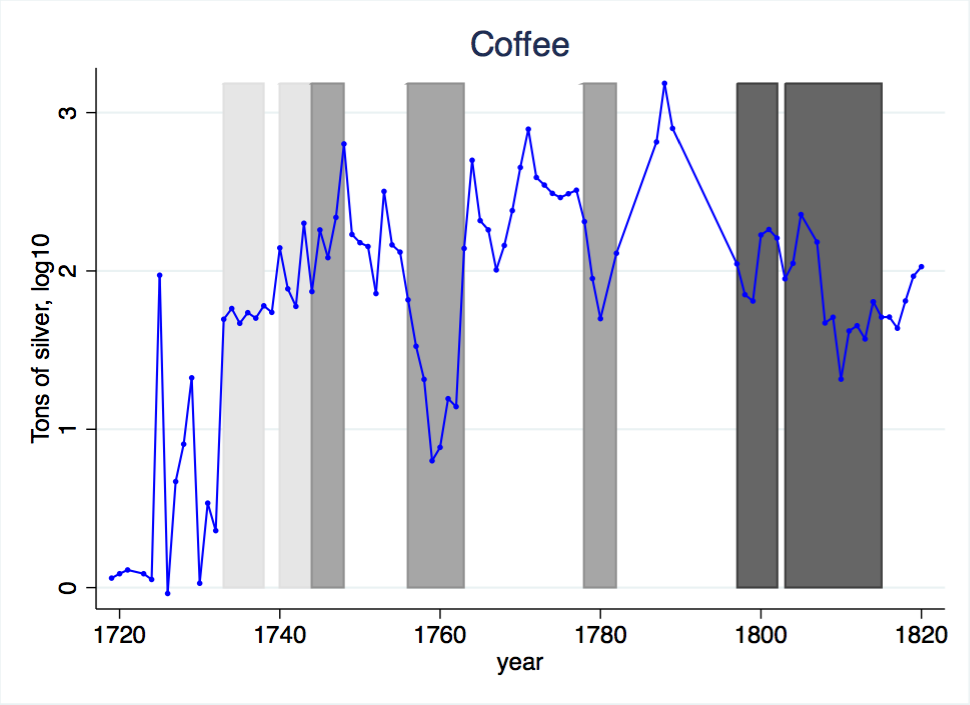
\includegraphics[scale=.25]{class1_trend}
\hfil 
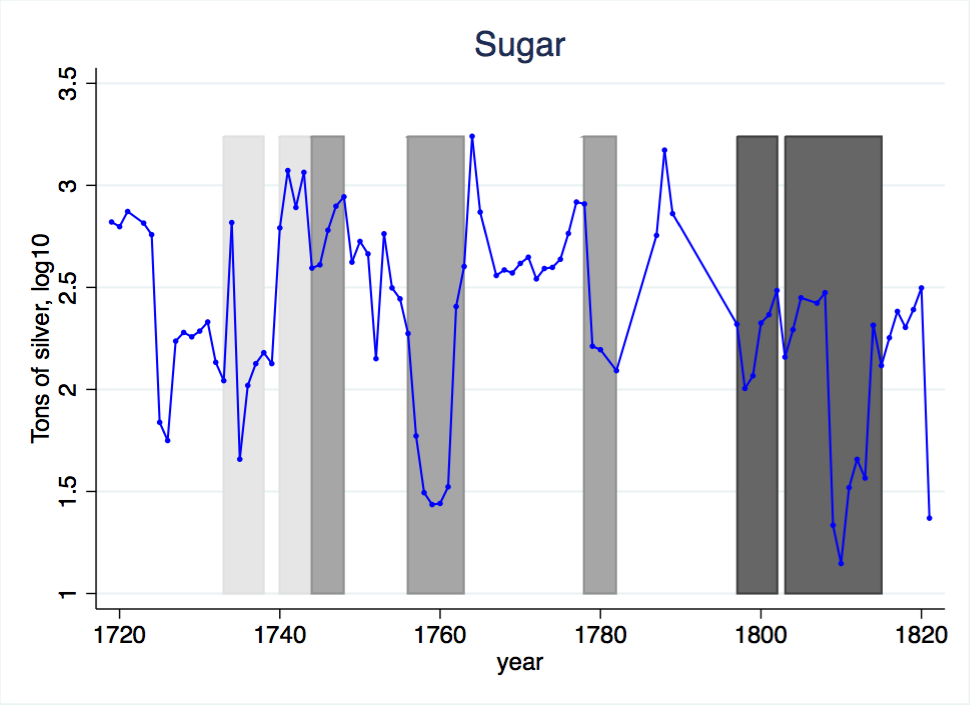
\includegraphics[scale=.25]{class3_trend}
\vspace*{.7em}
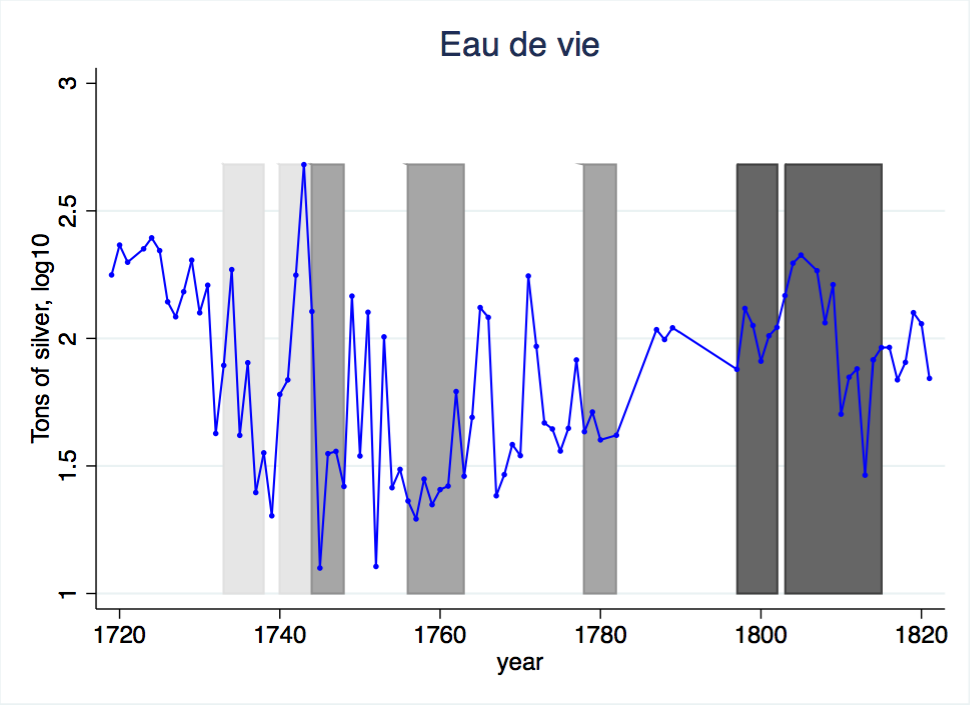
\includegraphics[scale=.25]{class2_trend}
\hfil 
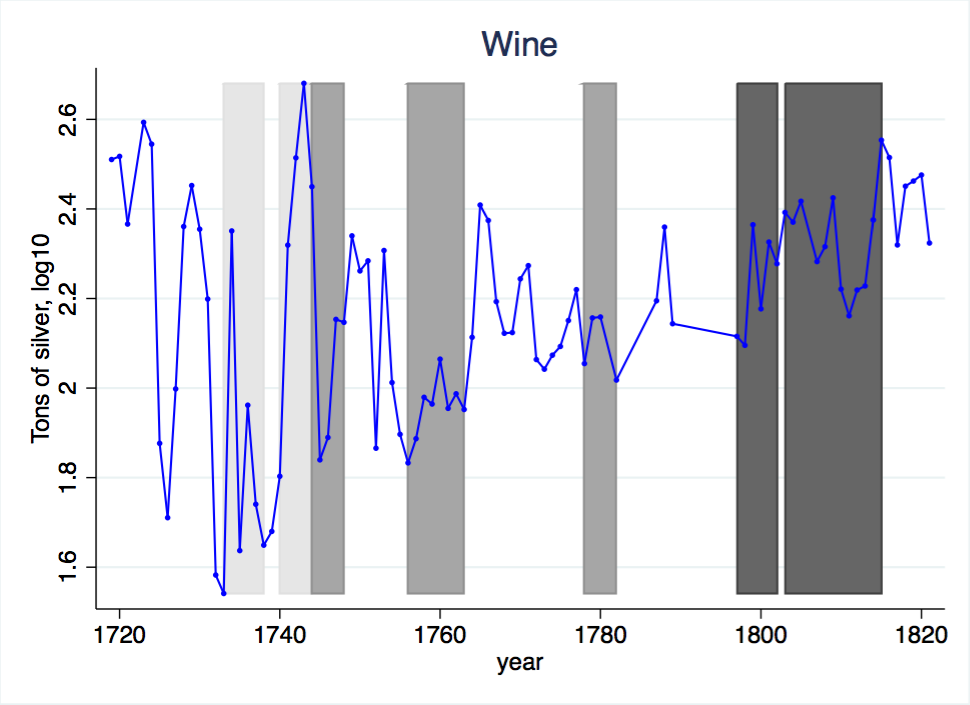
\includegraphics[scale=.25]{class4_trend}
\end{center}

\iffalse
\subsection{War lags}
In line with this reasoning, we turned next to analyse and compare war lags in the Hamburg case and general case. we run two regressions with and without product differentiation and for all wars together and a dummy for each war: 
\begin{multline}
\ln(exports_{i,t})=\beta_0+\beta_1country_i+\beta_2country_iyear+\beta_3adversaries_i+\beta_4neutral_i+\\+\beta_5adversary_ilag+\beta_6neutral_ilag+\beta_8allies_ilag
\end{multline}
\begin{multline}
\ln(exports_{i,t})=\beta_0+\beta_1country_i+\beta_2country_iyear+\beta_3product_{i,j}+\beta_4product_jyear+\\+\beta_5product_jadversary+ \beta_6product_jneutral+\beta_7product_jadversary_ilag+\beta_8neutral_ilag+\beta_9allies_ilag
\end{multline}

Results are quite in line with those seen in the Hamburg series. There is no post war negative coefficient, but on the contrary, trade increases by 40\% and 47\% in the first and second year after the war. Starting from the third year this effect decreases and coefficients are still positive but smaller. \\
Product-wise there is evidence of positive post war effects for all the products but in particular European products increase stably for the first four years after the war. War by war, we notice an interesting pattern after Seven Years War; exports of European goods increases as for the general case, but here we see that trade of sugar as well expands right after the war (+62\%). This is quite an interesting result given that sugar was, with coffee, the product which suffered the most during this conflict. 
In sum, we can say that, as for the case of Hamburg, there is no clear evidence of war lags, for sure not 10 years lag as claimed by Glick and Taylor (2005). Trade was extremely adaptive to conflicts in eighteenth century and neutral countries did not seem to suffer strong consequences.
we have also run the regression checking for pre war effects. Results are positive but very small in size for the general case, except for the case of allies countries, which has larger and more significant coefficients. The war-by-war case (considered all in one regression) is also not very meaningful; coefficients for Seven Years War are negative whereas those for American Revolutionary War are positive. In terms of difference between products, the results are again not very interesting. There is no stable pattern for pre war effect, except for coffee, which always shows an increase for all the four years preceding the war. However this might be just due to the increasing trend shown by coffee, disregarding the effects of wars.
Overall, for neutral countries the compensation effect is more likely as a post war phenomenon rather than a pre war one, again as noted for the case of Hamburg. 
\fi

\section{Robustness check}
We have also run some robustness check both for the Hamburg case and the general case. We have done so by using a log linear specification specification instead of the poisson pseudo maximum likelihood. \\
We have re-run all regressions mentioned in section 4 and 5, so both for Hamburg only and for all export destinations together. In the Hamburg aggregate case, the effects of wars are still negative and it is still possible to distinguish between colonial and non-colonial conflicts. While looking at the breakdown by products despite the fact that there is still a strong impact for colonial goods, no significant impact is found for wine and eau de vie, whose coefficients are negative and positively respectively, but insignificant. In the all-countries case on the other hand, the picture remains quite unchanged, and while the effect on coffee and sugar is strongly negative and significant, the effect on eau de vie is again positive and significant, even though less high, and wine is negative but small and insignificant. When turning to the aggregate case, results are very robust to the different specification and the effects are, once more, quite similar to the baseline case. \\
In addition to this, given the limited number of observations available in the Hamburg series at aggregate level, we have re-run the regression on the disaggregate export value by product, by adding product fixed effects to the regressions, but without interacting them with the war dummies. Table is shown in the appendix. The results of this different specification change a bit the picture in terms of colonial and non colonial wars, with non colonial wars resulting more disruptive that the colonial ones. The effect of the Polish war is also greater and that of the Seven years war is smaller.\\
Finally, as we have mentioned before, for the all-countries case with the product breakdown, we have relaxed the assumption of product time trend across countries and run a regression with country-product time trend. In both cases, the results are extremely close. In the regression with one dummy for all wars, coffee and sugar are nearly unchanged, only eau de vie and wine are a bit less positive. In the war-by-war case, results stay approximately the same, with the first three wars with a generalised strong effect and the last four with alternate effects on the different products. All tables are to be found in the appendix in the appendix.

\section{Conclusion}
In this paper we have analysed the effects of conflicts on neutral countries, taking Hamburg as a case study, and then compared our findings with the general case of all countries together. At aggregate yearly level, the impact of conflict on trade found for Hamburg looks much higher than the general case. To inspect this phenomenon, we then broke down the value of the series in four different products plus one category encompassing all other goods, and we checked for the impact on those specific products. We found that the difference between products is quite striking; colonial products suffer a bust in trade but trade of some European product even increased during conflicts. We have also checked for the difference in effects according to each kind of war, and in the case of Hamburg there is indeed evidence of a stronger effect of colonial wars on colonial products and of European wars on non-colonial products. This pattern however is not evident in the general case and we could not really disentangle the effects of the different kind of wars in a clear way. The results on the single products however, are robust to different specifications and it is indeed the case that some goods experienced a trade expansion in correspondence to conflicts and the collapse of other products. \\
We have also validated our results with several robustness check, including different Poisson Maximum Likelihood and log-linear specification but our findings do not change significantly. It would be interesting to aggregate countries to according to their export composition rather than their belligerent status and see whether our findings are still valid, but we leave this to further research. 
In conclusion, we are pointing out the fact that our results are quite different from those found in the literature so far, because we are using an example from another historical period. Most scholars treating this subject have used twentieth century data and generalized their findings to the overall history, disregarding the fact that twentieth century had brought major variations in many aspects. Wars had changed dramatically and their disruptive power had increased incredibly in the contemporary period. For this reason, results found in the literature so far are not robust to an extension over a longer time span, and with our contribution we intend to fill this gap. We believe that this work, by increasing the variety of the landscape of the observed effects of wars, might help to shed more light on the general mechanisms that link conflicts and commerce.


\pagebreak

\renewcommand{\baselinestretch}{1.0}\normalsize

\bibliographystyle{plainnat}
\bibliography{Futility_of_Mercantilist_Wars}




\end{document}



%\begin{thebibliography}{9}
%
%\bibitem{}
%Reuven Glick, Alan M. Taylor 
%\textit{Collateral damage: trade disruption and the economic impact of war}. 
%The Review of Economics and Statistics, February 2010, 92(1): 102–127
%
%\bibitem{}
%J. C. Riley
%\textit{The Seven Years War and the Old Regime in France}. 
%Series: Princeton Legacy Library, 1986, Published by: Princeton University Press, Pages: 280
%
%\bibitem{}
%Ahmed S. Rahman
%\textit{Fighting the Forces of Gravity - Seapower and Maritime Trade between the 18th and 20th Centuries}. 
%Explorations in Economic History Volume 47, Issue 1, January 2010, Pages 28–48
%
%
%\bibitem{}
%Rafael Reuveny. 
%\textit{Bilateral Import, Export, and Conflict/Cooperation Simultaneity}. 
%International Studies Quarterly, Vol. 45, No. 1 (Mar., 2001), pp. 131-158
%
%\bibitem{}
%Guillaume Daudin. 
%\textit{Domestic trade and market size in late eighteen century France}. 
%The Journal of Economic History / Volume 70 / Issue	03 / September 2010, pp 716-743
%
%
%\bibitem{}
%S. Brock Blomberg, Gregory D. Hess
%\textit{How much does violence tax trade?}. 
%The Review of Economics and Statistics (Impact Factor:2.66). 11/2006; 88(4):599:612
%
%\bibitem{}
%Charles H. Anderton, John R. Carter
%\textit{The Impact of War on Trade: An Interrupted Times-Series Study}. 
%2001 Journal of Peace Research, vol. 38, no. 4, 2001, pp. 445–457
%
%\bibitem{}
%Loic Charles and Guillaume Daudin
%\textit{Eighteen century international trade statistics sources and method}. 
%Revue de l’OFCE
%
%\bibitem{}
%Katherine Barbieri and Jack S. Levy
%\textit{Sleeping with the Enemy: The Impact of War on Trade}. 
%Journal of Peace Research, Vol. 36, No. 4, Special Issue on Trade and Conflict (Jul., 1999), pp. 463-479
%
%\bibitem{}
%Jennings
%\textit{Les marches du Nord dans le commerce francais au xvme siecle}. 
%Rennes, Presses Universitaires de Rennes, 2006, 390 p
%
%
%\bibitem{}
%Ahmed S. Rahman, Darrell J. Glaser
%\textit{Ex Tridenti Mercatus?- Sea-power and Maritime Trade in the Age of Globalization}. 
%Journal of International Economics Volume 100, May 2016, Pages 95–111
%
%\bibitem{}
%Ahmed S. Rahman
%\textit{Fighting the Forces of Gravity - Seapower and Maritime Trade between the 18th and 20th Centuries}. 
%Explorations in Economic History Volume 47, Issue 1, January 2010, Pages 28–48
%
%\bibitem{}
%Scott L. Baier, Jeffrey H. Bergstrand
%\textit{Do free trade agreements actually increase members' international trade?} 
%Journal of International Economics 71 (2007) 72–95
%
%\bibitem{}
%Philip Martin, Thierry Mayer, Mathias Thoenig
%\textit{Make Trade Not War?} 
%Review of Economic Studies (2008) 75, 865–900
%
%\bibitem{}
%Mary Lindemann
%\textit{The merchants republics: Amsterdam, Antwerp and Hamburg 1648-1790} 
%Cambridge:	Cambridge University Press, 2015. 374 pp. ISBN 978-1-107-07443-9.
%
%\bibitem{}
%S. Brock Blomberg, Gregory D. Hess , and Siddarth Thacker
%\textit{On the conflict-poverty nexus} 
%ECONOMICS \&\ POLITICS 0954-1985 Volume 18 November 2006 No.3
%
%\bibitem{}
%Patrick Villiers
%\textit{Marine Royale, corsaires et trafic dans l'Atlantique de Louis XIV à Louis XVI} 
%Diffusion Septentrion, Press universitaires, Thèse à la carte
%
%\bibitem{}
%Francois Crouzet
%\textit{La guèrre économique franco-anglaise au XVIII siècle} 
%Paris, ed. Fayard, 2008 ISBN 978-2-213-63601-6
%
%\bibitem{}
%Charles Carrière
%\textit{Negociants marseillais au XVIII siècle} 
%Marseille, A. Robert, 1973. 2 vol. gr. in-8, 1.111 pages. (Institut historique de Provence.)
%
%\bibitem{}
%Pierrick Pourchasse
%\textit{Le commerce du Nord. Les échanges commerciaux entre la France et l’Europe septentrionale au XVIIIe siècle, Rennes} Presses Universitaires de Rennes, 2006, 390 p., ISBN 978-2753500976.
%
%\bibitem{}
%Lagerqvist L. and E Nathorst-Boos, 
%\textit{Mynt}, Bokforlaget PAN /Norstedts, Stockholm, 1968, p.78
%
%\bibitem{}
%Anne Husted Burleigh
%\textit{John Adams} American presidents series, Transaction Publishers 2009, p. 189
%
%\bibitem{}
%Griffiths, David M. \textit{An American Contribution to the Armed Neutrality of 1780.} Russian Review 30, no. 2 (April 1971).
%
%\end{thebibliography}
%
